\documentclass[init,francais,RandD]{rapportPFE}
\usepackage{listings}
\usepackage{indentfirst}
\usepackage{eurosym}
\usepackage{chronosys}

\titre{Navigation et contrôle multi-robots pour l'inspection acoustique de structures métalliques}
\title{Multi-robot navigation and control for acoustic inspection of metal plate structures}
\firstname{Brandon}
% \middlename{Jérémy}
\lastname{Alves}
\dateDebutPFE{9 janvier 2023}
\dateFinPFE{30 juin 2023}
\nomStructureAcceuil{INRIA}
\villeStructureAccuel{Villeurbanne, France}
% \logoStructureAccueil{width=1.5cm}{graphics/LogoStructureAccueil}
\begin{encadrants}
	\referent{Référent}{Olivier \Nom{Simonin}}{Professeur}{INSA Lyon}
	\tuteur{Référent}{Cédric \Nom{Pradalier}}{Professeur}{Georgia Tech Europe}
	\tuteur{Tuteur}{Mathieu \Nom{Maranzana}}{Maître de conférences}{INSA Lyon}
\end{encadrants}
\date{\today}

\begin{document}
	\maketitle
	\begin{ResumeMotsCles}
		% abstract no more than 12 lines.
		\begin{resumeEn}
			This project is part of the European project BugWright2, which aims to address the problem of inspecting large metal structures using heterogeneous fleets of mobile robots. The project will focus on developing navigation strategies for mobile robots using guided ultrasonic waves to perform the inspection of metal plates. Guided waves have the ability to propagate along a plate by interacting with the material that makes it up and being affected by changes in geometry, such as corrosion. By combining measurements between a transmitter and a distant receiver system, it is possible to perform a tomography of the area to be inspected and potentially identify and locate points of corrosion.
		\end{resumeEn}
		\keywords{Navigation~; Multi-Robot~; Tomography~; Ultrasonic Guided Waves~; Inspection.}
		% Résumé pas plus de 12 lignes
		\begin{resumeFr}
			Ce projet fait partie du projet européen BugWright2 qui a pour objectif de résoudre la problématique de l'inspection de grandes structures métalliques en utilisant des flottes hétérogènes de robots mobiles. Le projet se concentrera sur le développement de stratégies de navigation pour des robots mobiles utilisant des ondes ultrasoniques guidées pour réaliser l'inspection de plaques métalliques. Les ondes guidées ont la capacité de se propager le long d'une plaque en interagissant avec la matière qui la compose et en étant affectées par des changements de géométrie, tels que la corrosion. En combinant des mesures entre un système émetteur et un système récepteur distant, il est possible de réaliser une tomographie de la zone à inspecter et de potentiellement identifier et localiser des points de corrosion.
		\end{resumeFr}
		\motscles{Navigation~; Multi-Robot~; Tomographie~; Ondes Guidées Ultrasoniques~; Inspection.}
	\end{ResumeMotsCles}
		% \begin{remerciements}
		%   Merci à tous. Commenter cet environnement s'il n'est pas nécessaire.
		% \end{remerciements}
	\setcounter{tocdepth}{3}
	\tableofcontents
	\cleardoublepage
	\section{Introduction}
		%Contexte,
		Ce projet de fin d'étude s'inscrit dans le contexte plus large du projet européen BugWright2, qui vise à résoudre la problématique de l'inspection autonome et la maintenance de grandes structures métalliques avec des flottes hétérogènes de robots mobiles. Dans ce projet, nous nous concentrons sur le développement de stratégies de navigation pour un ensemble de robots mobiles utilisant des ondes ultrasoniques guidées pour réaliser l'inspection des plaques métalliques. En effet, les ondes guidées ont la particularité de se propager le long d'une plaque en interagissant avec la matière qui la compose, et en étant affectées par des changements de géométrie liés, en particulier, à la corrosion.

		%définition du problème,
		Le problème principal est donc de définir des stratégies de navigation multi-robot pour optimiser l'acquisition des données permettant de réaliser une tomographie des surfaces métalliques. Pour atteindre cet objectif, nous allons dans un premier temps effectuer une recherche bibliographique, puis mettre en place des méthodes de navigation dans un environnement de simulation. Enfin, nous envisagerons un déploiement sur différents robots en fonction des résultats obtenus. Ce projet sera réalisé sous la supervision de Olivier Simonin (INSA Lyon CITI lab) et de Cédric Pradalier (CNRS IRL2958 GT).

		%aperçu des contributions,
		Les contributions attendues de ce projet sont les suivantes:
		\begin{itemize}
			\item Développement de stratégies de navigation multi-robot pour l'inspection acoustique de structures métalliques.
			\item Optimisation de l'acquisition de données pour la réalisation de la tomographie.
			\item Résolution des problèmes de coordination entre les robots et de synchronisation des horloges.
			\item Implémentation des méthodes de navigation dans un environnement de simulation et leur déploiement sur des robots réels.
		\end{itemize}

		%plan du rapport
		Dans ce dossier d'initialisation, nous présenterons le projet de fin d'étude avec son contexte, objectifs et environnement scientifique et technique. Nous discuterons également de l'organisation du projet de fin d'étude avec notamment les livrables attendus ainsi que le planning. Enfin nous présenterons les risques et les moyens de les gérer.
	\section{Présentation du Projet de Fin d'Études}
		\subsection{Contexte}
			Le projet BugWright2 est un projet européen qui vise à résoudre la problématique de l'inspection des grandes structures métalliques, de type coques de bateaux, avec des flottes hétérogènes de robots mobiles. BugWright2 est un projet d'une durée approximative de 4 ans. Il a commencé le 01/01/2020 et doit se terminer le 31/03/2024. Ce projet est coordonné par C. Pradalier et implique de nombreux partenaires. Son coût totale s'élève à 9 952 745.63\euro{}, dont 8 999 807.50\euro{} financé par l'union européenne. Le contexte général de ce projet est donc l'inspection de structures métalliques, qui est un enjeu important pour la maintenance et la sécurité des infrastructures. Il est à noter que, bien que le domaine d'application de ce projet soit l'inspection de coques de bateaux, les méthodes développées pourront être utilisées pour d'autres applications, de type surfaces métalliques relativement planes. Une illustration des différents robots utilisés dans ce projet est présentée dans la figure \ref{fig:cartoon}, où l'on peut y voir des drones, des crawlers ainsi que des AUV (Autonomous Underwater Vehicle).

			\begin{figure}[h]
				\centering
				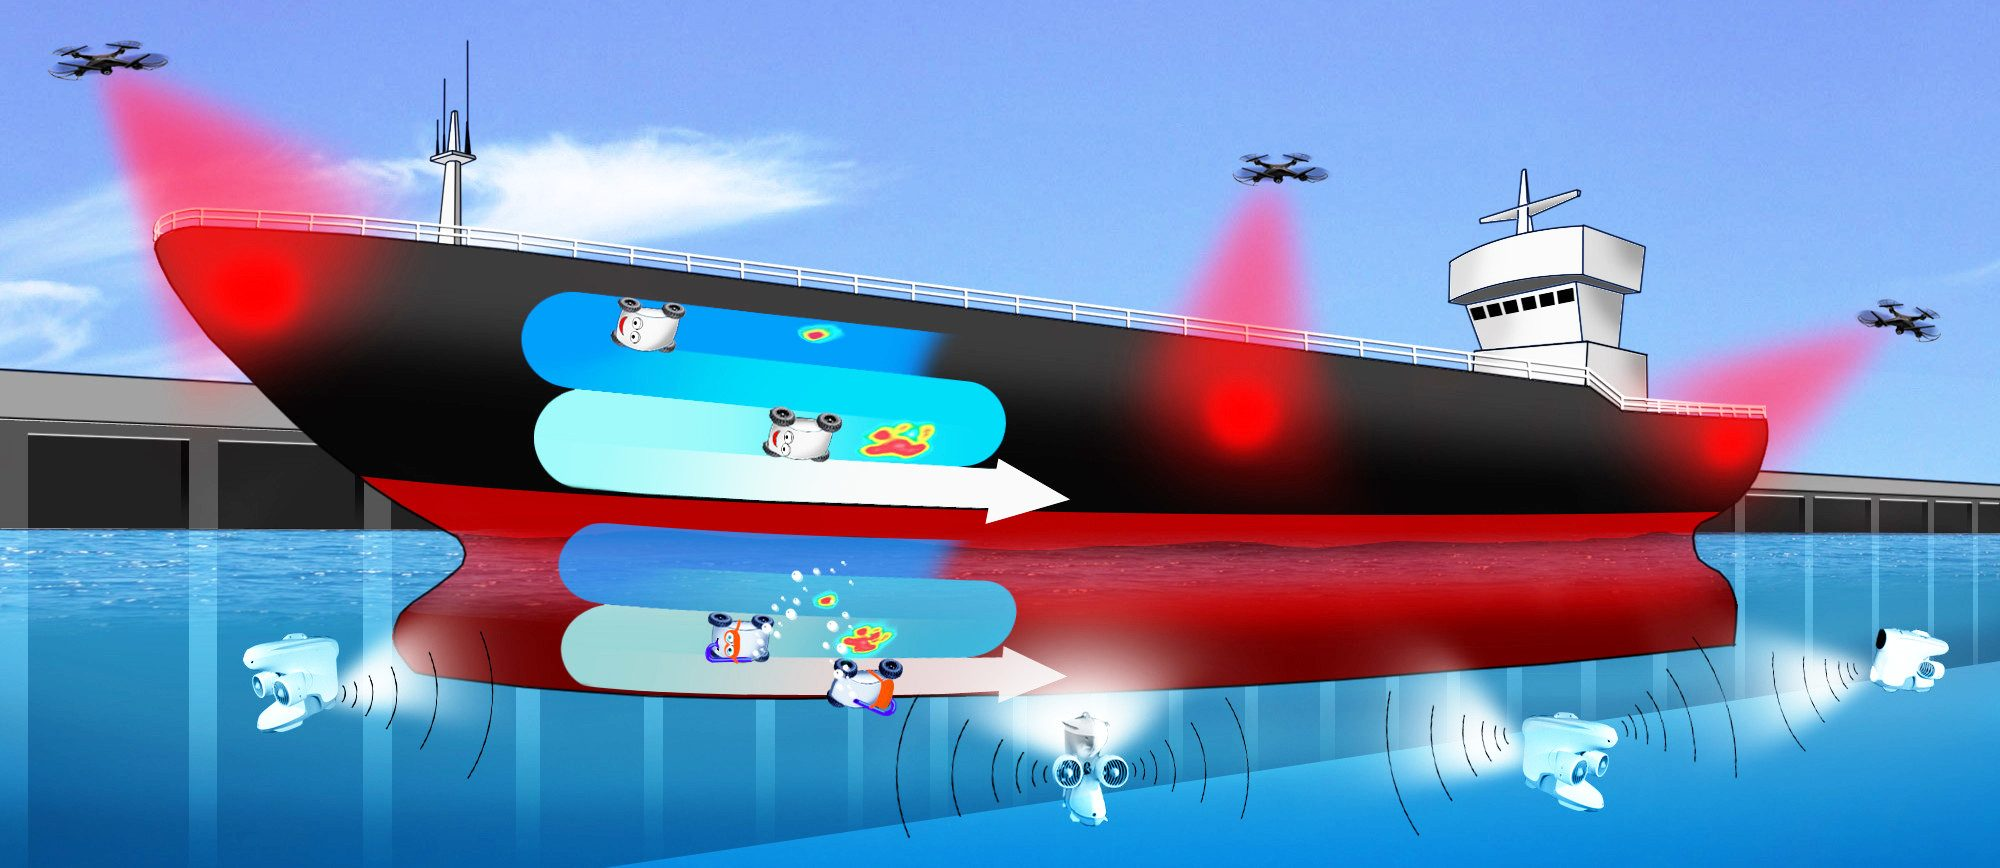
\includegraphics[width=0.8\textwidth]{graphics/Concept-Cartoon-NJ3-e1582812224528.jpg}
				\caption{Illustration des robots utilisés dans le projet BugWright2.}
				\label{fig:cartoon}
			\end{figure}

			Dans ce projet, nous nous concentrons plus particulièrement sur l'utilisation de robots mobiles et d'ondes ultrasoniques guidées pour réaliser l'inspection de plaques métalliques. Les ondes ultrasoniques guidées ont la particularité de se propager le long d'une plaque en interagissant avec la matière qui la compose, et en étant affectées par des changements de géométrie liés, en particulier, à la corrosion. Ainsi, en positionnant un robot émetteur et un robot récepteur sur la plaque, on peut émettre des ondes ultrasoniques et les recevoir à l'aide du récepteur. Dans le cas où les ondes ultrasoniques traverseront des zones de corrosion, elles seront perturbées et le receveur pourra détecter ces perturbations. Une estimation des zones de corrosion pourra alors être réalisée.

			Cette technique permet donc de réaliser une tomographie de la zone à inspecter et potentiellement d'identifier et de localiser des points de corrosion. Cependant, cela nécessite de connaître précisément la position de l'émetteur et du récepteur ainsi que de synchroniser les horloges des deux entités.

			Les robots utilisés seront des robots de type Crawler, qui sont des robots mobiles à roues métalliques. Une illustration de ces robots est présentée dans la figure \ref{fig:robots}. Ces robot ont la perticularité de s'accrocher aux plaques métalliques et de pouvoir se déplacer sur ces dernières. Les capteurs d'ondes ultrasoniques guidées peuvent leur permettre de détecter des zones de corrosion plus précisément que des drones, dans le cas où c'est zones de corrosion ne serait pas visible par les caméras des drones. Ces types de robots sont donc particulièrement adaptés à une inspection précise de grandes surfaces métalliques.

			Enfin, dans ce projet de fin d'études, les surfaces que nous considéront sont des surfaces métalliques planes (2D). Une carte des zones de corrosion devra donc être produite à partir des données collectées par les robots. Cette carte pourra être utilisée pour localiser les zones de corrosion et ainsi permettre de réaliser des réparations plus précises.

			\begin{figure}[h]
				\centering
				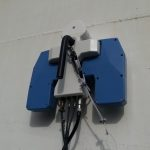
\includegraphics[width=0.2\textwidth]{graphics/altiscan_closeup-150x150.jpg}
				\caption{Illustration des robots crawlers utilisés dans le projet.}
				\label{fig:robots}
			\end{figure}
		\subsection{Objectifs}
			L'objectif principal de ce projet est de définir des stratégies de navigation multi-robot pour optimiser l'acquisition de données permettant de réaliser la tomographie des structures métalliques, tout en résolvant les problèmes de communication et de coordination entre les robots.

			Pour atteindre cet objectif global, il est prévu de réaliser les tâches suivantes:
			\begin{itemize}
				\item Effectuer une recherche bibliographique sur les techniques de navigation multi-robot pour l'inspection acoustique de structures métalliques.
				\item Développer des stratégies de navigation multi-robot pour l'inspection acoustique de structures métalliques.
				\item Mettre en place des méthodes de navigation dans un environnement de simulation.
				\item Optimiser l'acquisition de données pour la réalisation de la tomographie. L'exploration des robots et la prise de données devront minimiser un coût qui sera le temps de navigation et de prise de données des robots.
				\item Résoudre les problèmes de coordination entre les robots.
				\item Envisager un déploiement sur des robots réels en fonction des résultats obtenus dans l'environnement de simulation.
			\end{itemize}
		\subsection{Environnement scientifique et technique.}
			Ce projet de fin d'étude s'inscrit dans le domaine de la robotique, plus précisément dans celui de la navigation multi-robot pour l'inspection acoustique de structures métalliques. Il implique également la mise en œuvre d'ondes ultrasoniques guidées pour réaliser cette inspection.

			Pour cela, les méthodes de navigation multi-robot seront développées en utilisant des outils de simulation de robotique. Ces outils permettront de simuler la mobilité des agents robotiques et les mesures entre agents. Les outils de simulation utilisés seront Gazebo et Rviz. ROS (Robot Operating System) 1 sera également utilisé pour l'implémentation des différentes stratégies de navigation multi-robot. Les algorithmes de navigation seront développés en C++ et Python. Les algorithmes de navigation seront testés dans l'environnement de simulation et éventuellement sur des robots réels.

			Le projet sera mené en collaboration avec l'équipe d'Olivier Simonin de l'INSA Lyon et de Cédric Pradalier de l'IRL2958 GT-CNRS à Metz. L'équipe de l'INSA Lyon fournira l'expertise sur les environnements de simulations robotiques. Le laboratoire GT-CNRS à Metz sera utilisé pour la partie expérimentale. L'équipe CHROMA de l'INSA Lyon, supervisée par Olivier Simonin, est notamment composée de deux ingénieurs qui sont respectivement spécialisés sur Gazebo et ROS.
	\section{Organisation}
		\subsection{Livrables}
			Les livrables attendus de ce projet de fin d'étude sont les suivants:
			\begin{itemize}
				\item Livrables PFE
				\begin{itemize}
					\item Un rapport de projet détaillant les recherches effectuées, les méthodes développées, les résultats obtenus et les conclusions. Ce rapport devra inclure une description détaillée des algorithmes de navigation développés et une analyse des résultats obtenus lors des tests en simulation et éventuellement sur des robots réels.
					\item Les codes source des algorithmes de navigation développés, qui devront être commentés et documentés de manière à permettre une compréhension facile et une réutilisation éventuelle.
					\item Une présentation orale sur les résultats obtenus.
				\end{itemize}
				\item Livrables Laboratoire
				\begin{itemize}
					\item Un état de l'art sur les techniques de navigation multi-robots pour l'inspection acoustique de structures métalliques.
					\item Des démonstrations vidéos des simulations ou des tests sur des robots réels.
					\item Des fiches de lectures des articles scientifiques étudiés dans le cadre de ce projet.
				\end{itemize}
			\end{itemize}
		\subsection{Planning}
			Il est important de définir clairement les étapes clés du projet ainsi que les échéances pour chacune d'elles, afin de s'assurer que le projet se déroule de manière efficace et organisée. Le planning prévisionnel comprendra les étapes suivantes :
			\begin{enumerate}
				\item Recherche bibliographique : cette étape consistera à effectuer une recherche approfondie sur les travaux existants en matière de navigation multi-robots pour l'inspection acoustique de structures métalliques. Cette étape commencera en début de projet et aura une duréé approximative d'un mois (du 09/01/2023 au 09/02/2023).
				\item Développement des algorithmes : une fois la recherche bibliographique terminée, cette étape consistera à développer les algorithmes de navigation multi - robots adaptés à l'inspection acoustique de structures métalliques. Cette étape commencera à la suite de la recherche bibliographique et aura une durée approximative de 3 mois (du 09/02/2023 au 01/05/2023).
				\item Simulation : les algorithmes développés seront testés dans un environnement de simulation pour évaluer leur performance. Cette étape commencera en parallèle du développement des algorithmes et aura une durée approximative de 3 mois (du 09/02/2023 au 01/05/2023).
				\item Tests expérimentaux : si les résultats de la simulation sont concluants, les algorithmes seront ensuite testés sur des robots réels. La mise en pratique de la simulation sur des robots réels pourra être affectée par des contraintes techniques comme par exemple du bruit au niveau des capteurs ou des problèmes de communication. Cette étape commencera à la suite de la simulation et aura une durée approximative de 1 mois (du 01/05/2023 au 01/06/2023).
				\item Rapport de fin d'étude : cette étape consistera en la rédaction d'un rapport détaillant les travaux effectués, les résultats obtenus et les contributions à la recherche. Cette étape commencera à la suite des tests expérimentaux et aura une durée approximative de 1 mois (du 01/06/2023 au 30/06/2023).
			\end{enumerate}
			Il est important de noter que ces étapes ne sont pas nécessairement linéaires et qu'il peut y avoir des retours en arrière pour apporter des améliorations ou des modifications aux algorithmes développés.
	\section{Gestion des risques}
		Cette section, consacrée à la gestion des risques, a pour objectif de définir les risques potentiels liés au projet et de proposer des mesures pour les minimiser ou les éviter. Il est important d'identifier les risques en amont afin de pouvoir les gérer efficacement et de s'assurer que le projet se déroule de manière efficace et organisée.

		Dans le cadre de ce projet de fin d'étude, plusieurs risques ont été identifiés et seront pris en compte pour minimiser leur impact sur le déroulement et les résultats du projet. Nous avons identifié les risques suivants:
		\begin{itemize}
			\item L'incapacité à développer des algorithmes de navigation fiables et précis. Pour minimiser ce risque, nous allons tester et valider nos algorithmes sur des véhicules simulés avant de les implémenter sur un véhicule réel.
			\item Le manque de temps pour terminer le projet. Pour minimiser ce risque, nous allons suivre un planning détaillé et faire des révisions régulières pour s'assurer que nous restons sur la bonne voie.
			\item Le manque de compétences en matière de robotique. Pour minimiser ce risque, nous allons nous appuyer sur les compétences de l'équipe de l'INSA Lyon et de l'IRL2958 GT-CNRS à Metz.
			\item Le manque de compétences en matière de simulation. Pour minimiser ce risque, nous allons nous appuyer sur les compétences de l'équipe de l'INSA Lyon.
		\end{itemize}
		En mettant en place des mesures pour minimiser ces risques, nous nous efforçons de garantir la réussite de notre projet de navigation autonome.
	\section{Conclusion}
		En conclusion, ce projet de fin d'étude vise à développer des stratégies de navigation multi-robot pour optimiser l'acquisition de données permettant de réaliser une tomographie de la zone à inspecter, avec des ondes ultrasoniques guidées pour réaliser l'inspection de plaques métalliques. Nous avons défini les objectifs de ce projet, les livrables attendus, le planning et les risques potentiels pour ce projet. Nous sommes convaincus que les résultats de ce projet contribueront au développement de l'inspection automatique de structures métalliques en utilisant des flottes hétérogènes de robots mobiles.
	% Bibliographie
	% Annexes éventuelles (en plus des 30 pages demandées)
	% \bibliographystyle{unsrt}
	% \bibliography{rapportPFE}
\end{document}
